
\chapter{The \algo\ Algorithm}
In this chapter, we introduce the main contribution of this paper: the Clustered-Graph Rule Generation (CGRG) algorithm. The \algo\ algorithm derives association rules from a clustered minimum spanning tree. The input to the algorithm is a minimum spanning tree, where the vertices are a set of items and the edges are the associations between them. Section \ref{sec:clustering} describes how the minimum spanning tree is segmented into clusters. Using these clusters, Section \ref{sec:itemsets} details how itemsets for the rules will be generated from these clusters. Sections \ref{sec:bicluster} and \ref{sec:intracluster} describe how the algorithm will generate two distinct classes of rules (bi-cluster and intra-cluster, respectively). Section \ref{sec:prune} describes how the rules will then be pruned such that only the statistically significant rules will remain.
Figure \ref{fig:algorithm_flow} illustrates the complete flow for the \algo\ algorithm.
\begin{figure}[H]
\centering
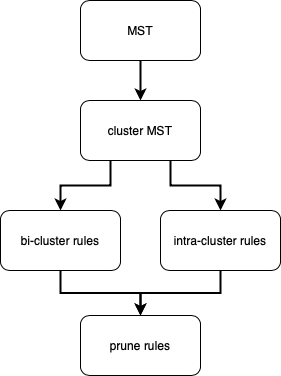
\includegraphics[scale=0.6]{ruleflow}
\caption{\algo\ algorithm}
\label{fig:algorithm_flow}
\end{figure}


\section{Markov Clustering}
\label{sec:clustering}
The MST will be clustered using the Markov Clustering (MCL) algorithm.
\pcite{modularity} defined a measure $Q$ of a network's partition into distinct communities (i.e. of its modularity).
Multiple cluster configurations will be generated using the algorithm with varying inflation scores to identify the most modular configuration\footnote{Where the connectedness between dense clusters is minimal}, which will then be used to segment the MST.


\section{Itemset Generation}
\label{sec:itemsets}
For every cluster $Cl_i$ identified by the MCL algorithm, all proper subsets $cl$ such that $cl \subseteq Cl_i$ are generated. The set of proper subsets are stored against the key $i$, which denotes the index of cluster $Cl_i$, effectively assigning each cluster its proper subsets. Listing \ref{lst:itemset_generation} is the pseudo-code for this operation.
\begin{lstlisting}[language=C, mathescape=true, caption=Cluster Itemset Generation, label=lst:itemset_generation]
given CLUSTERS = {$Cl_1, Cl_2,\dots,Cl_n$}
define itemsets_by_cluster as {$\emptyset$}
for $Cl_i$ in CLUSTERS
    to items_by_cluster add ({all $cl$ if $cl \subseteq Cl_i$} at index $i$)
\end{lstlisting}

\section{Bi-Cluster Rule Generation}
\label{sec:bicluster}
Bi-cluster rules are those where the antecedent and the consequent originate from distinct and separate clusters. All possible bi-cluster rules are generated such that for any two given clusters $Cl_k$ and $Cl_j$:
\[
cl_k \rightarrow cl_j;\;\; cl_k \subseteq Cl_k, \; cl_j \subseteq Cl_j
\]
Listing \ref{lst:bicluster} presents the pseudo-code for the bi-cluster rule generation. All bi-cluster combinations are generated and stored as a pair of indices (i.e. $(i,j)$ for clusters $Cl_i$ and $Cl_j$). For every cluster pair generated, every configuration of itemsets associated with each cluster (calculated in Listing \ref{lst:itemset_generation}) is added to the ruleset such that a rule exists for every itemset $cl_k$ associated with cluster $Cl_k$ and every itemset $cl_j$ associated with cluster $Cl_j$.

\begin{minipage}{\linewidth}
\begin{lstlisting}[language=C, mathescape=true, caption=Bi-Cluster Rule Generation, label=lst:bicluster]
given CLUSTERS = {$Cl_1, Cl_2,\dots,Cl_n$}
given itemsets_by_cluster = {$\dots$} // already populated
define rules as $\emptyset$
define combs as $\emptyset$
to combs add all $^nC_2$ combinations from {$1,2,\dots,n$}

for comb in combs:
    define antecedent_itemsets as (itemsets_by_cluster at (c at index 1)) // first index is 1
    define consequent_itemsets as (itemsets_by_cluster at (c at index 2))
    for antecedent in antecedent_itemsets:
        for consequent_item in consequent:
            to rules add (antecedent $\rightarrow$ consequent)
            to rules add (consequent $\rightarrow$ antecedent)
\end{lstlisting}
\end{minipage}

\section{Intra-Cluster Rule Generation}
\label{sec:intracluster}
Intra-cluster rules are those where itemsets in both the antecedent and consequent originate from the same cluster. This can be represented as:
\[
cl_{k1} \rightarrow cl_{k2}; \;\;\;\; cl_{k1} \subseteq Cl_k,\; cl_{k2} \subseteq Cl_k,\; cl_{k1} \cap cl_{k2} = \emptyset
\]

\begin{lstlisting}[language=C, mathescape=true, caption=Intra-Cluster Rule Generation, label=lst:intracluster]
given CLUSTERS = {$Cl_1, Cl_2,\dots,Cl_n$}
given itemsets_by_cluster = {$\dots$} // already populated
define rules as $\emptyset$
for $i$ in itemsets_by_cluster
    define itemsets as (itemsets_by_cluster at index i) // itemsets at $i^{th}$ cluster.
    define combs = $\emptyset$
    to combs add all $^pC_2$ combinations from itemsets // For all p elements in itemsets
    
    for comb in combs
        define antecedent as (comb at index 1) // first index is 1
        define consequent as (comb at index 2)
        to rules add (antecedent $\rightarrow$ consequent)
        to rules add (consequent $\rightarrow$ antecedent) 
\end{lstlisting}
Listing \ref{lst:intracluster} is the pseudo-code for the intra-cluster rule generation. A rule is generated from every configuration of two subsets from the subsets of a given cluster.

\section{Rule Pruning}
\label{sec:prune}
\begin{lstlisting}[language=C, mathescape=true, caption=Rule Pruning, label=lst:prune]
given rules = {$\dots$}                 // already populated
sort rules ascending by antecedent // sort by number of items in antecedent
define min_support as float        // user-specified value
define min_confidence as float     // user-specified value
define valid_rules as $\emptyset$
define below_threshold as $\emptyset$
for r in rules
    antecedent = (r at index 1) // first index is 1
    consequent = (r at index 2)
    define is_above_threshold = True 
    // check if support lookup can be skipped
    for itemset in below_threshold
        if itemset $\subset$ r
            is_above_threshold = false
            break
    if is_above_threshold
        // calculate all supports
        define support_antecedent as float
        define support_consequent as float
        define support_r as float 
        define confidence as (support_r $\div$ support_antecedent)
        define lift as (confidence $\div$ support_consequent)
        if support_antecedent < min_support
            to below_threshold add support_antecedent
        if support_consequent < min_support
            to below_threshold add support_consequent
        if confidence < min_confidence:
            next loop // move to next rule in for loop
        if support_r < min_support
            next loop 
        // If all constraints met, add rule
        to valid_rules add r
\end{lstlisting}
Listing \ref{lst:prune} presents the pseudo-code for rule pruning, employing the use of the \textit{Apriori Principle} described in Section \ref{sec:ais}, which states that \textit{the support of a set is - at most - equal to the support of its subsets}.
We first sort the rules in ascending order by the number of items in the antecedent of each rule, so that if any itemsets with only a few items are found to be below our constraints, we can ignore any larger itemsets where those same items are present.
When iterating through the rules, if the support of either the antecedent or consequent is found to be below the user specified support constraint, it is added \texttt{below\_threshold} - the set of itemsets found to be below our constraint. For every subsequent iteration, if it is found that any set from \texttt{below\_threshold} is a subset of the current rule, we can discard the rule and avoid having to calculate its support as we know it will be below our support constraint. Our final rules are those that remain after pruning.

\section{Overview}
To recap, the \algo\ algorithm segments the regions of the minimum spanning tree into distinct clusters by identifying dense clusters within the tree, and then produces rules where the antecedent and consequent of the rules originate from a cluster. The rules are then pruned to only include rules that satisfy our support and confidence constraints. Figure \ref{fig:algorithm_flow} outlines the steps in achieving the final rules.